\chapter[Eletrônica]{Eletrônica}


 
 A construção de uma máquina de venda autômoma de chopp depende da construção de diversos subsistemas,
 que correspondem aos requisitos do projeto. Assim, seguem os requisitos do projeto.

\begin{itemize}
\item Controle de temperatura
\item Abertura do reservatório de copos
\item Controle de saída de chopp
\end{itemize}
  
Os códigos utilizados neste trabalho encontram-se em controle de versão na ferramenta GitHub 
e podem ser facilmente acessados em: \url{https://github.com/autochopp/embedded_electronics}. 

\section{Requisitos do Projeto}

\begin{enumerate}
\item Controle de temperatua

\textbf{Dado} que a leitura da temperatura do sensor de temperatura

\textbf{Quando} a temperatura estiver fora da faixa estabelecida

\textbf{Então} acionar  relé de controle do compressor


\item Abertura do reservatório de copos

\textbf{Dado} que a leitura da temperatura do sensor seja maior 2ºC

\textbf{Quando} a temperatura estiver fora da faixa estabelecida

\textbf{Então} acionar ou não relé



\item Controle da saída de chopp

\begin{enumerate}

\item Indentificar a presença do copo na base

\textbf{Dado} que o usuário foi solicitado para colocar o copo na base 

\textbf{Quando} os contadores do \textit{timeout} se iniciarem

\textbf{Então} verificar se o copo se encontra na base 



\item Controlar a inclinação do copo

\textbf{Dado} que a compra foi liberada

\textbf{Quando} o copo se encontra na base

\textbf{Então} acionar motores que inclinam a base


\item Estimar volume de chopp no copo

\textbf{Dado} que o usuário escolheu um volume de copo

\textbf{Quando} houver tiragem de chopp

\textbf{Então} esperar o tempo necessário para tirar o volume esperado

\textbf{OU} esperar o sinal de parada do sensor de presença



\item Estimar volume restante no barril

\textbf{Dado} que se sabe o volume presente no barril em um dado instante

\textbf{Quando} houver tiragem de chopp

\textbf{Então} subtrair valor da tiragem do valor do valor do volume anterior



\item Garantir o colarinho escolhido

\textbf{Dado} que o usuário escolheu um determinado colarinho

\textbf{Quando} a compra foi liberada e o chopp foi  tirado

\textbf{Então} acionar ou não motor que controla o colarinho


\end{enumerate}

\end{enumerate}


\section{Casos de teste}

\section{Funcionamento}

A Figura \ref{state_machine} representa o funcionamento e a interação dos sistemas de eletrônica por meio
de uma máquina de estados. Nela, as etapas de liberação do copo, verificação da posição do copo, inclinação do copo,
tiragem do chopp, retorno do copo a posição inicial e inserção do colarinho são mostradas.

\begin{figure}[!htb]
            \centering
         	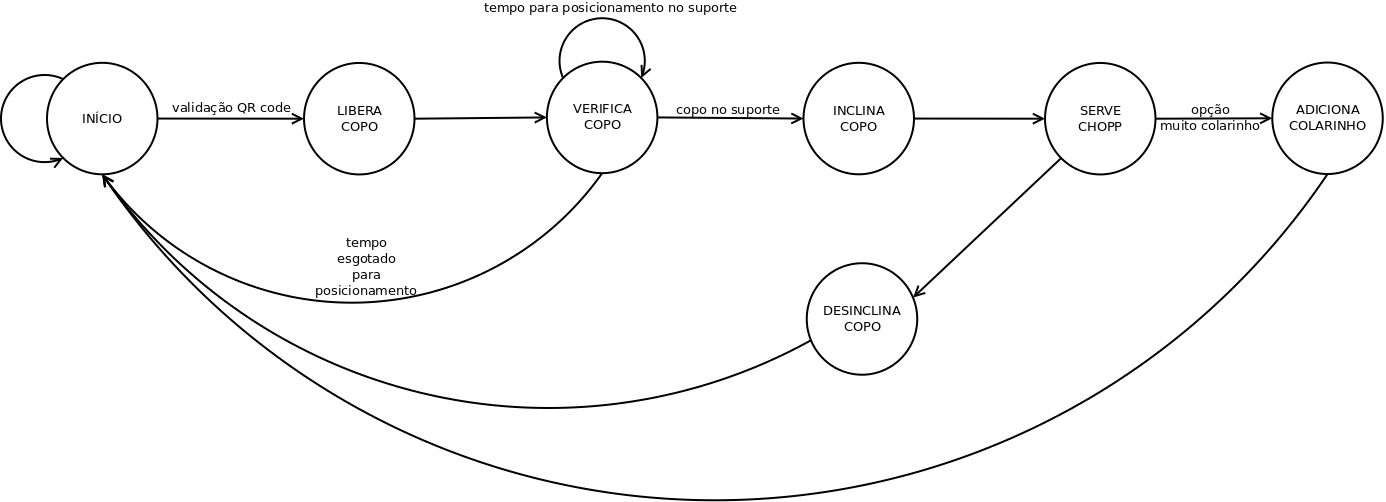
\includegraphics[scale= 0.25]{figuras/maquina_estado_eletronica.png}
            \caption{Máquina de estados que representa o funcionamento do subsistema de tiragem de chopp.}
            \label{state_machine}
\end{figure}
 
Inicialmente, a máquina aguarda a solicitação de tiragem de chopp, bem como a confirmação/autenticação de compra. 
Após ter isso confirmado, os dados referentes ao tipo de tiragem são processados (tamanho do copo, quantidade de colarinho
e tipo de chopp) e as configurações para uma tiragem correta são feitas.

Logo após isso, a máquina aciona a solenoide que libera o copo aprópriado ao tamanho de chopp selecionado e aguarda que o 
usuário  posicione o copo no suporte da máquina. O  sistema foi pensado de modo que o usuário tem um tempo limite para
posicionar o copo no suporte, após o qual a tiragem é desconsiderada e a máquina volta ao seu estado inicial de espera.

Caso o copo seja posicionado no suporte, inicia-se o processo de tiragem de chopp. Nesse processo, o suporte do copo é
inclinado por meio do acionamento do motor e a válvula que libera o chopp é acionada. Passa-se a próxima etapa no caso de um
de dois eventos ocorrer: o tempo máximo de tiragem ser excedido ou o 
volume tirado chegar ao limiar de altura estabelecido no copo.

Se o usuário tiver selecionado colarinho, o motor que libera uma maior entrada de ar no sistema e cria o colarinho é 
acionado. Após isso, a válvula de chopp é fechada, o copo retorna a sua 
posição inicial e máquina retorna ao seu estado de espera por uma nova requisição.

O sistema de refrigeração encontra-se funcionando independentemente dos processos de venda/tiragem de chopp e ocorre de forma
contínua e ininterrupta.

\section{Solução adotada}

\subsection{Controle de temperatura}

Para realizar o controle da temperatura, permitindo que o chopp esteja sempre gelado quando da retirada, 
é utilizado o sensor de temperatura DS18B20 presente na Figura \ref{sensor-temperatura}. 
Ele  permite a leitura de temperatura  mesmo em ambientes úmidos, tal qual esta aplicação. 
O sensor descrito mede temperaturas entre   $ -55 ^\circ C$ e $125 ^\circ C$ com erro de $\pm 0.5 ^\circ C$.
O sensor encontra-se posicionado na saída de chopp, que permite uma leitura mais fidedigna da
temperatura real do chopp, uma vez que  na saída o chopp já circulou por toda a serpentina e está em
equilíbrio térmico. O modo como esse sensor é conectado pode ser visto na Figura \ref{esquema-temperatura}.

\begin{figure}[!htb]
            \centering
         	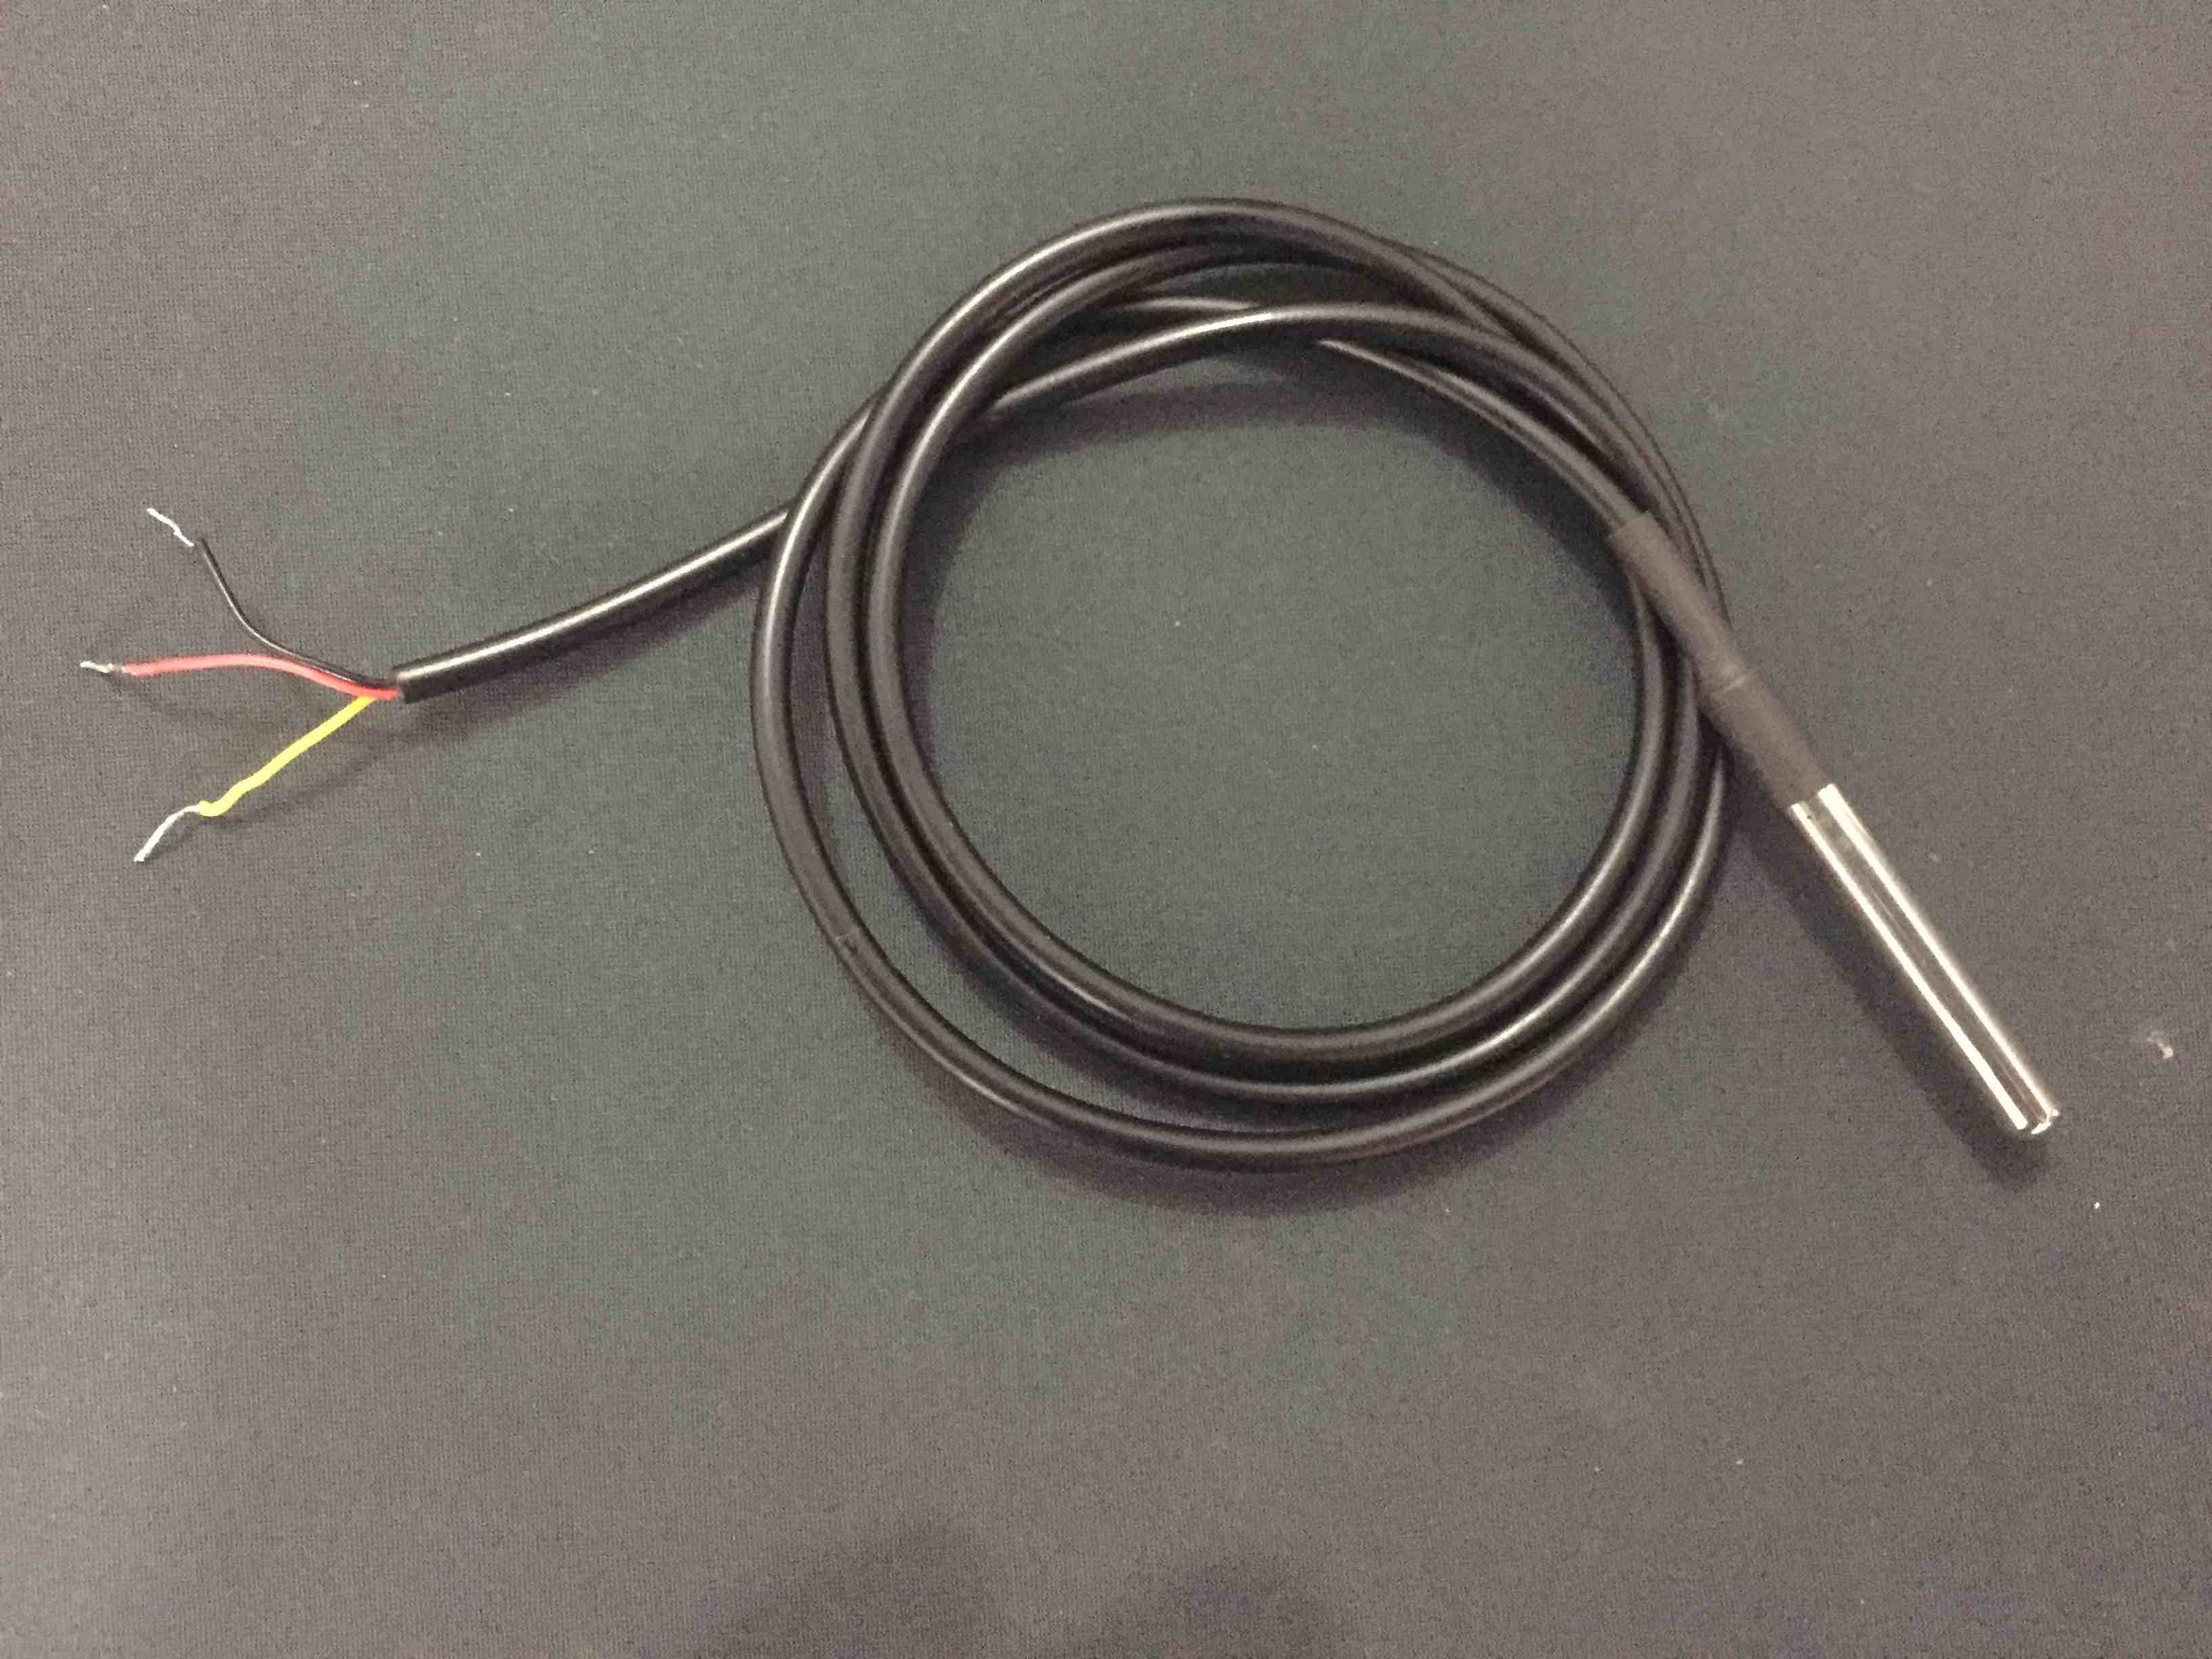
\includegraphics[scale= 0.08]{figuras/temperatura.jpg}
            \caption{Sensor de temperatura DS18B20. Fonte: Própria.}
            \label{sensor-temperatura}
\end{figure}
               
A medição da temperatura permite a ativação do compressor mantendo a temperatura na faixa
ideal entre $-1$ e $1 ^\circ C$. Tal ativação será realizada pelo acionamento de um módulo relé  
ligado ao compressor. 
    
\begin{figure}[!htb]
           \centering
           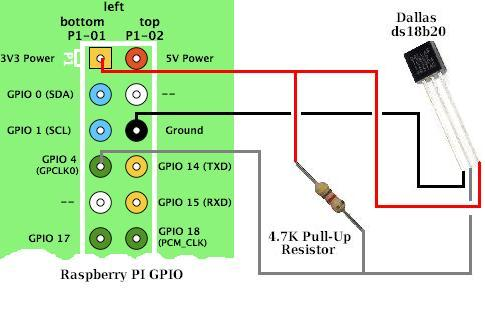
\includegraphics[scale= 0.5]{figuras/esquema.jpg}
            \caption{Esquemático do sensor de temperatura. Imagem da internet.}
            \label{esquema-temperatura}
\end{figure}    
    

\subsection{Controle de saída de chopp}

\subsubsection{Presença do copo}
Há a necessidade de se verificar a presença do copo no sistema para que o chopp possa ser tirado. 
Para tanto, inicialmente utilizou-se o sensor ultrassônico HC-SR04, porém, o mesmo inviabilizou seu
uso devido a complexidade de sua comunicação com o computador (\textit{Raspberry pi}).

Como solução mais direta e que evitaria tal nível de complexidade, optou-se por utilizar um sensor de trilha, 
que se comunica de forma direta com o computador e retorna um valor binário para a presença ou não do copo. 
Essa escolha traz como consequências a necessidade de uma tira branca no copo
 e a necessidade de uso de um copo transparente, para não interferir com os sensores.


\subsubsection{Estimar volume no copo}
Para que se pudesse ter um controle do volume presente no copo e consequentemente volume 
restante nos reservatórios, inicialmente pensou-se em utilizar dois sensores (por redundância), 
sendo eles o sensor de fluxo YFS201 e uma célula de carga.

Obtiveram-se resultados satisfatórios na montagem do sensor de fluxo, porém verificou-se um erro 
muito grande em suas medidas, o qual chegava a dez porcento nos testes efetuados. 
Já quanto ao sensor de carga, não houve sucesso em sua implementação, apresentando resultados quase que aleatórios.

Após discutir o presente problema com professores e orientadores, outra solução foi proposta.
A solução proposta se utiliza de diodos emissores de luz e fototransistores posicionados a 
uma distância conhecida. Sabendo-se a bitola do tubo utilizado e, contando-se o tempo entre 
os acionamentos, pode-se calcular o fluxo passante, porém também não se obteve sucesso nessa abordagem

A solução final encontrada foi se utilizar de sensores de trilha posicionados ao longo do copo, juntamente com um acionamento 
por tempo. O acionamento por tempo garante que não se passe do volume total do copo, em caso de falha,
e o sensores de trilha garantem o volume solicitado. Isso foi projetado de modo que se garantisse uma maior precisão e eficácia
na tiragem do chopp, dadas pelos sistemas redundantes.


\subsubsection{Garantir o colarinho escolhido}
O controle do colarinho é feito através da atuação de motores, estes  movimentam
a alavanca que controla a saída de chopp e colarinho. Desta forma é necessário realizar 
medições de tempo para cada tamanho de colarinho selecionável, servindo assim a quantidade. 
Esse acionamento é feito por tempo e relaciona-se com a entrada de ar no  sistema.


\subsection{Atuação dos motores}
Dois dos mais importantes subsistemas que contribuem diretamente com a experiência do usuário são 
a inclinação do copo e a tiragem automática do chopp, para tais tarefas fez-se o uso de motores de passo.
Para o controle dos motores usou-se dos pinos da \textit{Raspberry pi}.

Os motores precisam ser alimentados com 12V, para isso usa-se uma fonte de energia externa. Isso é dado pelo
 consumo de corrente dos motores, que é superior a aquela fornecida pelos pinos da \textit{Raspberry pi}. Assim,
fez-se necessário o uso de um \textit{driver} L298N. A Figura \ref{motor} mostra o sistema dos motores montado.

\begin{figure}[!h]
            \centering
         	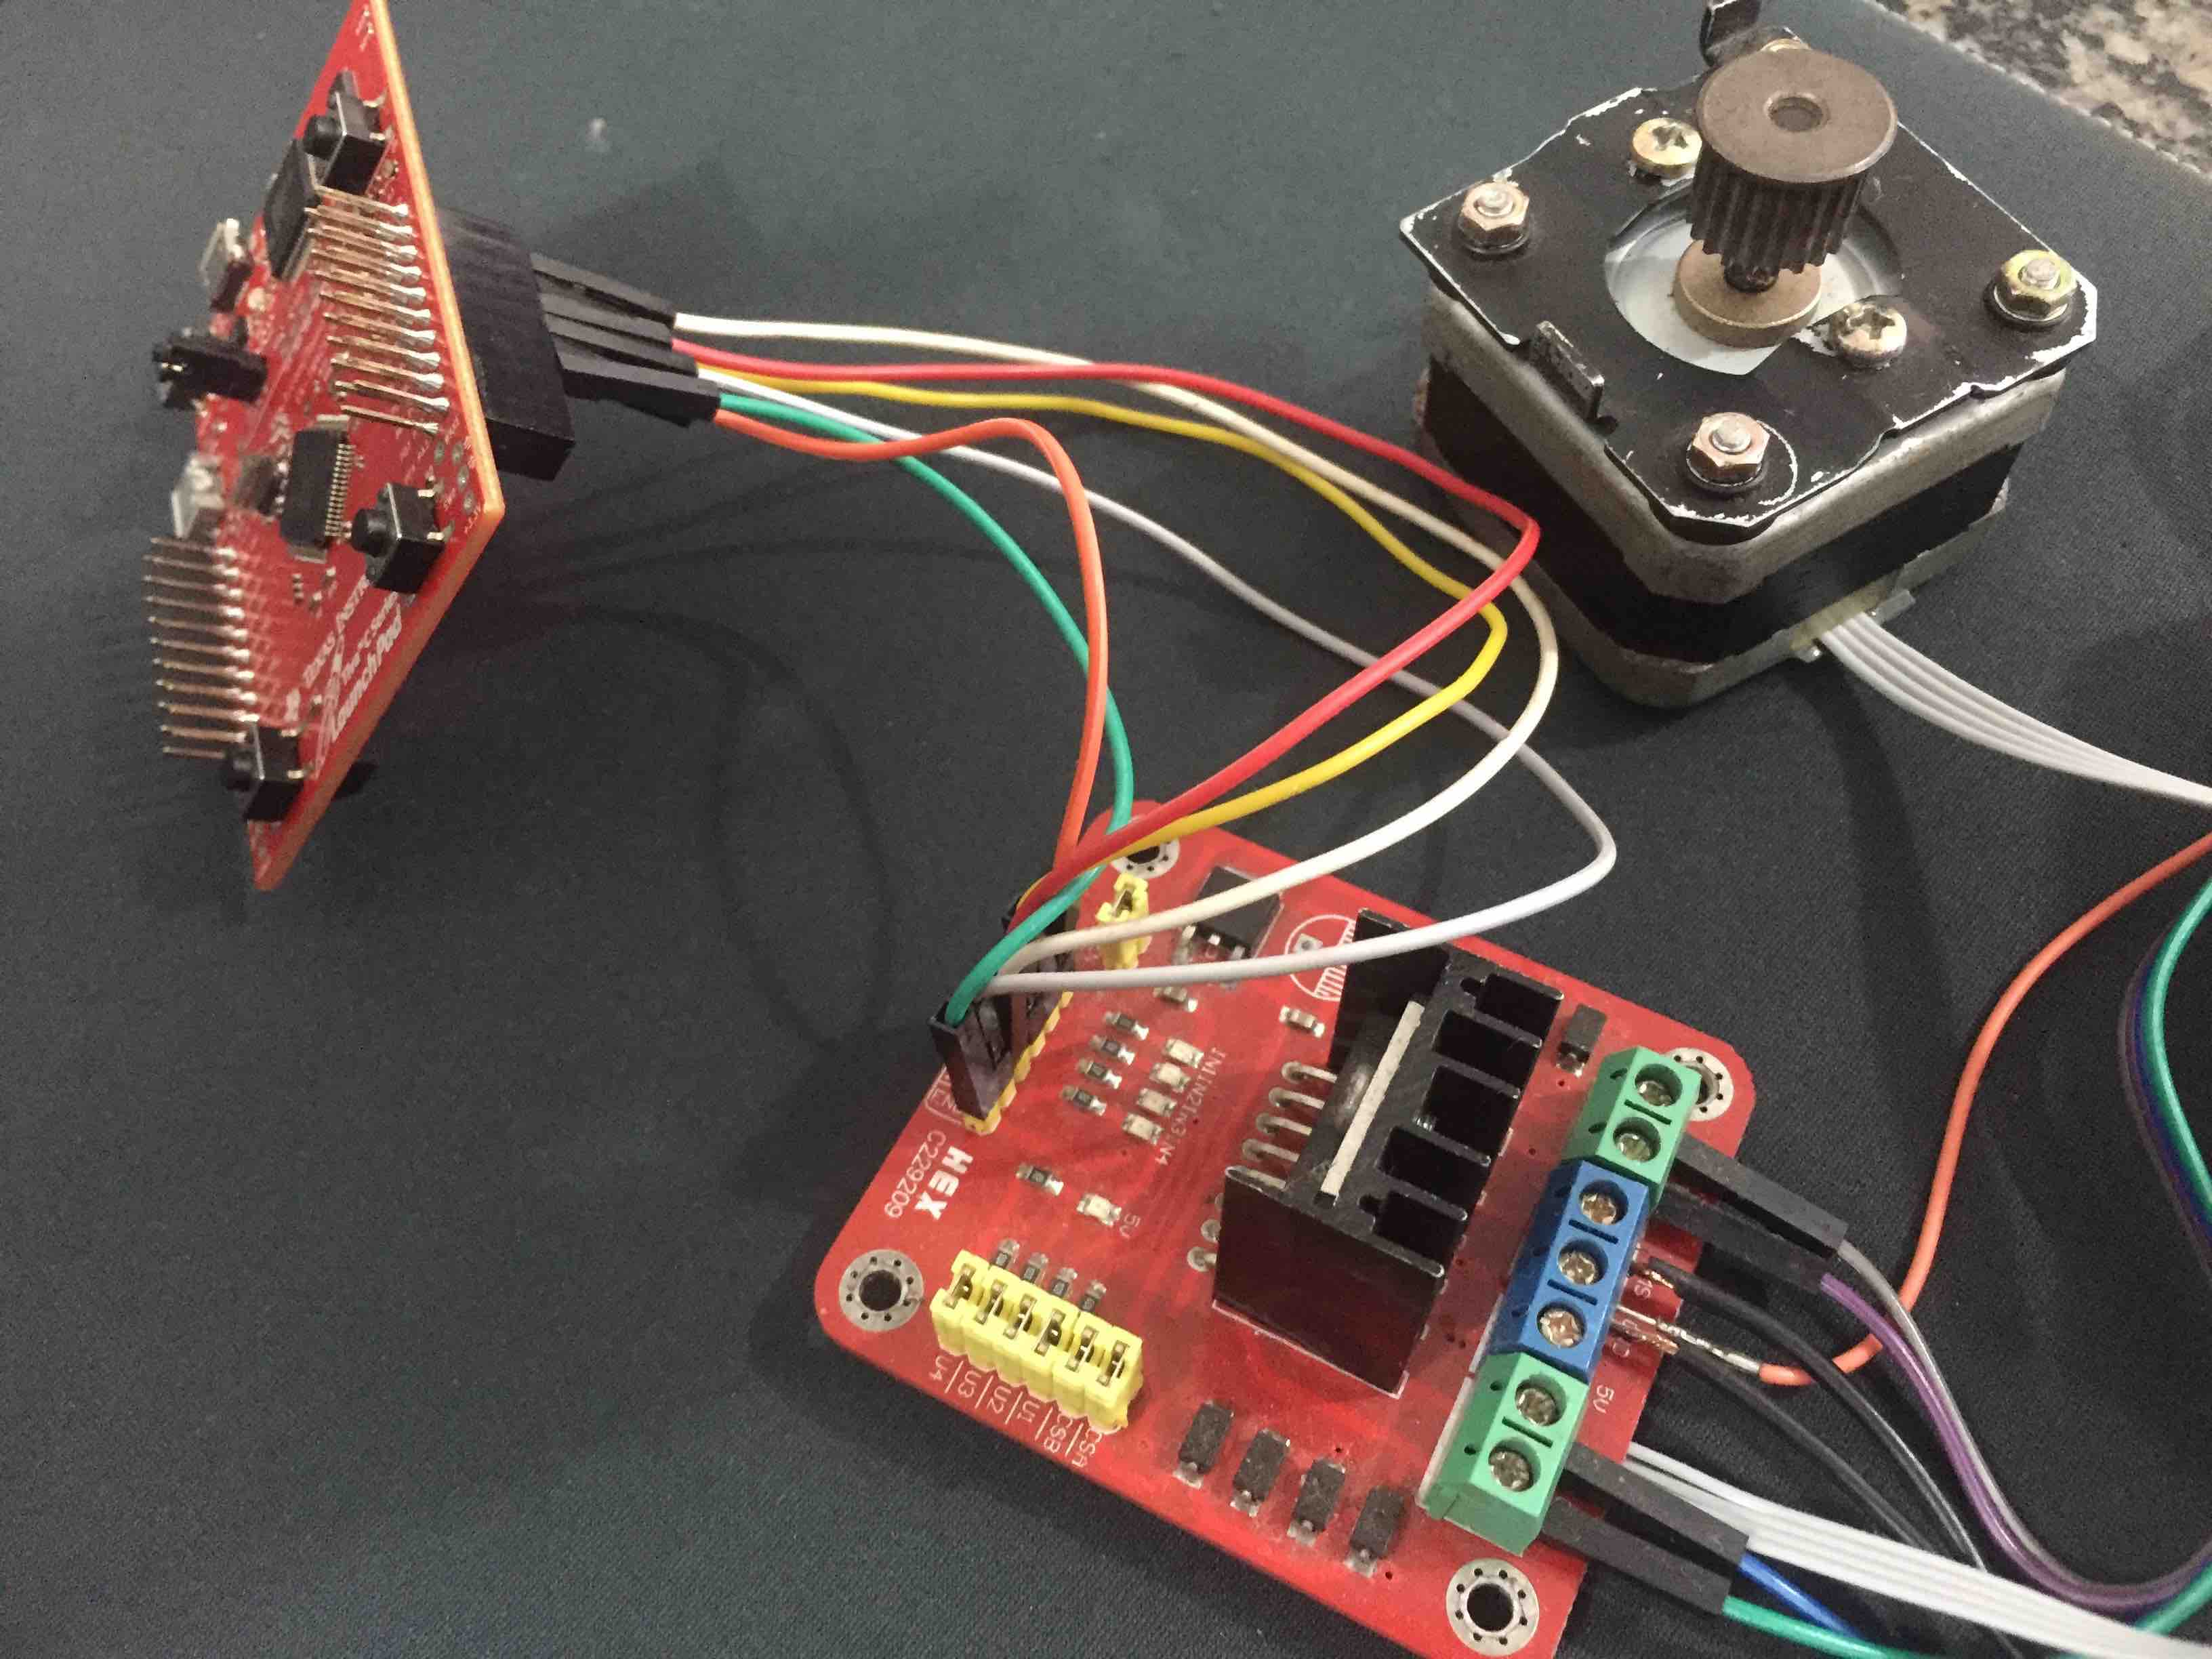
\includegraphics[scale= 0.08]{figuras/motor.jpg}
            \caption{Sistema de acionamento de motor de passo.}
            \label{motor}
\end{figure}

\newpage
\subsection{Abertura do reservatório de copos}

 Esse serviço se fez necessário, após a decisão de disponibilizar o copo ao usuário, 
 portanto os copos são  armazenados na própria máquina. Para disponibilizar os copos, 
 eles são dispostos de forma que sempre que exista uma requisição de um chopp, 
 um copo caia em um reservatório próprio. Para empurrar os copos são utilizados duas 
 solenoides de modelo TAU-0530, uma delas pode ser vista na Figura \ref{solenoide}. 

\begin{figure}[!h]
            \centering
         	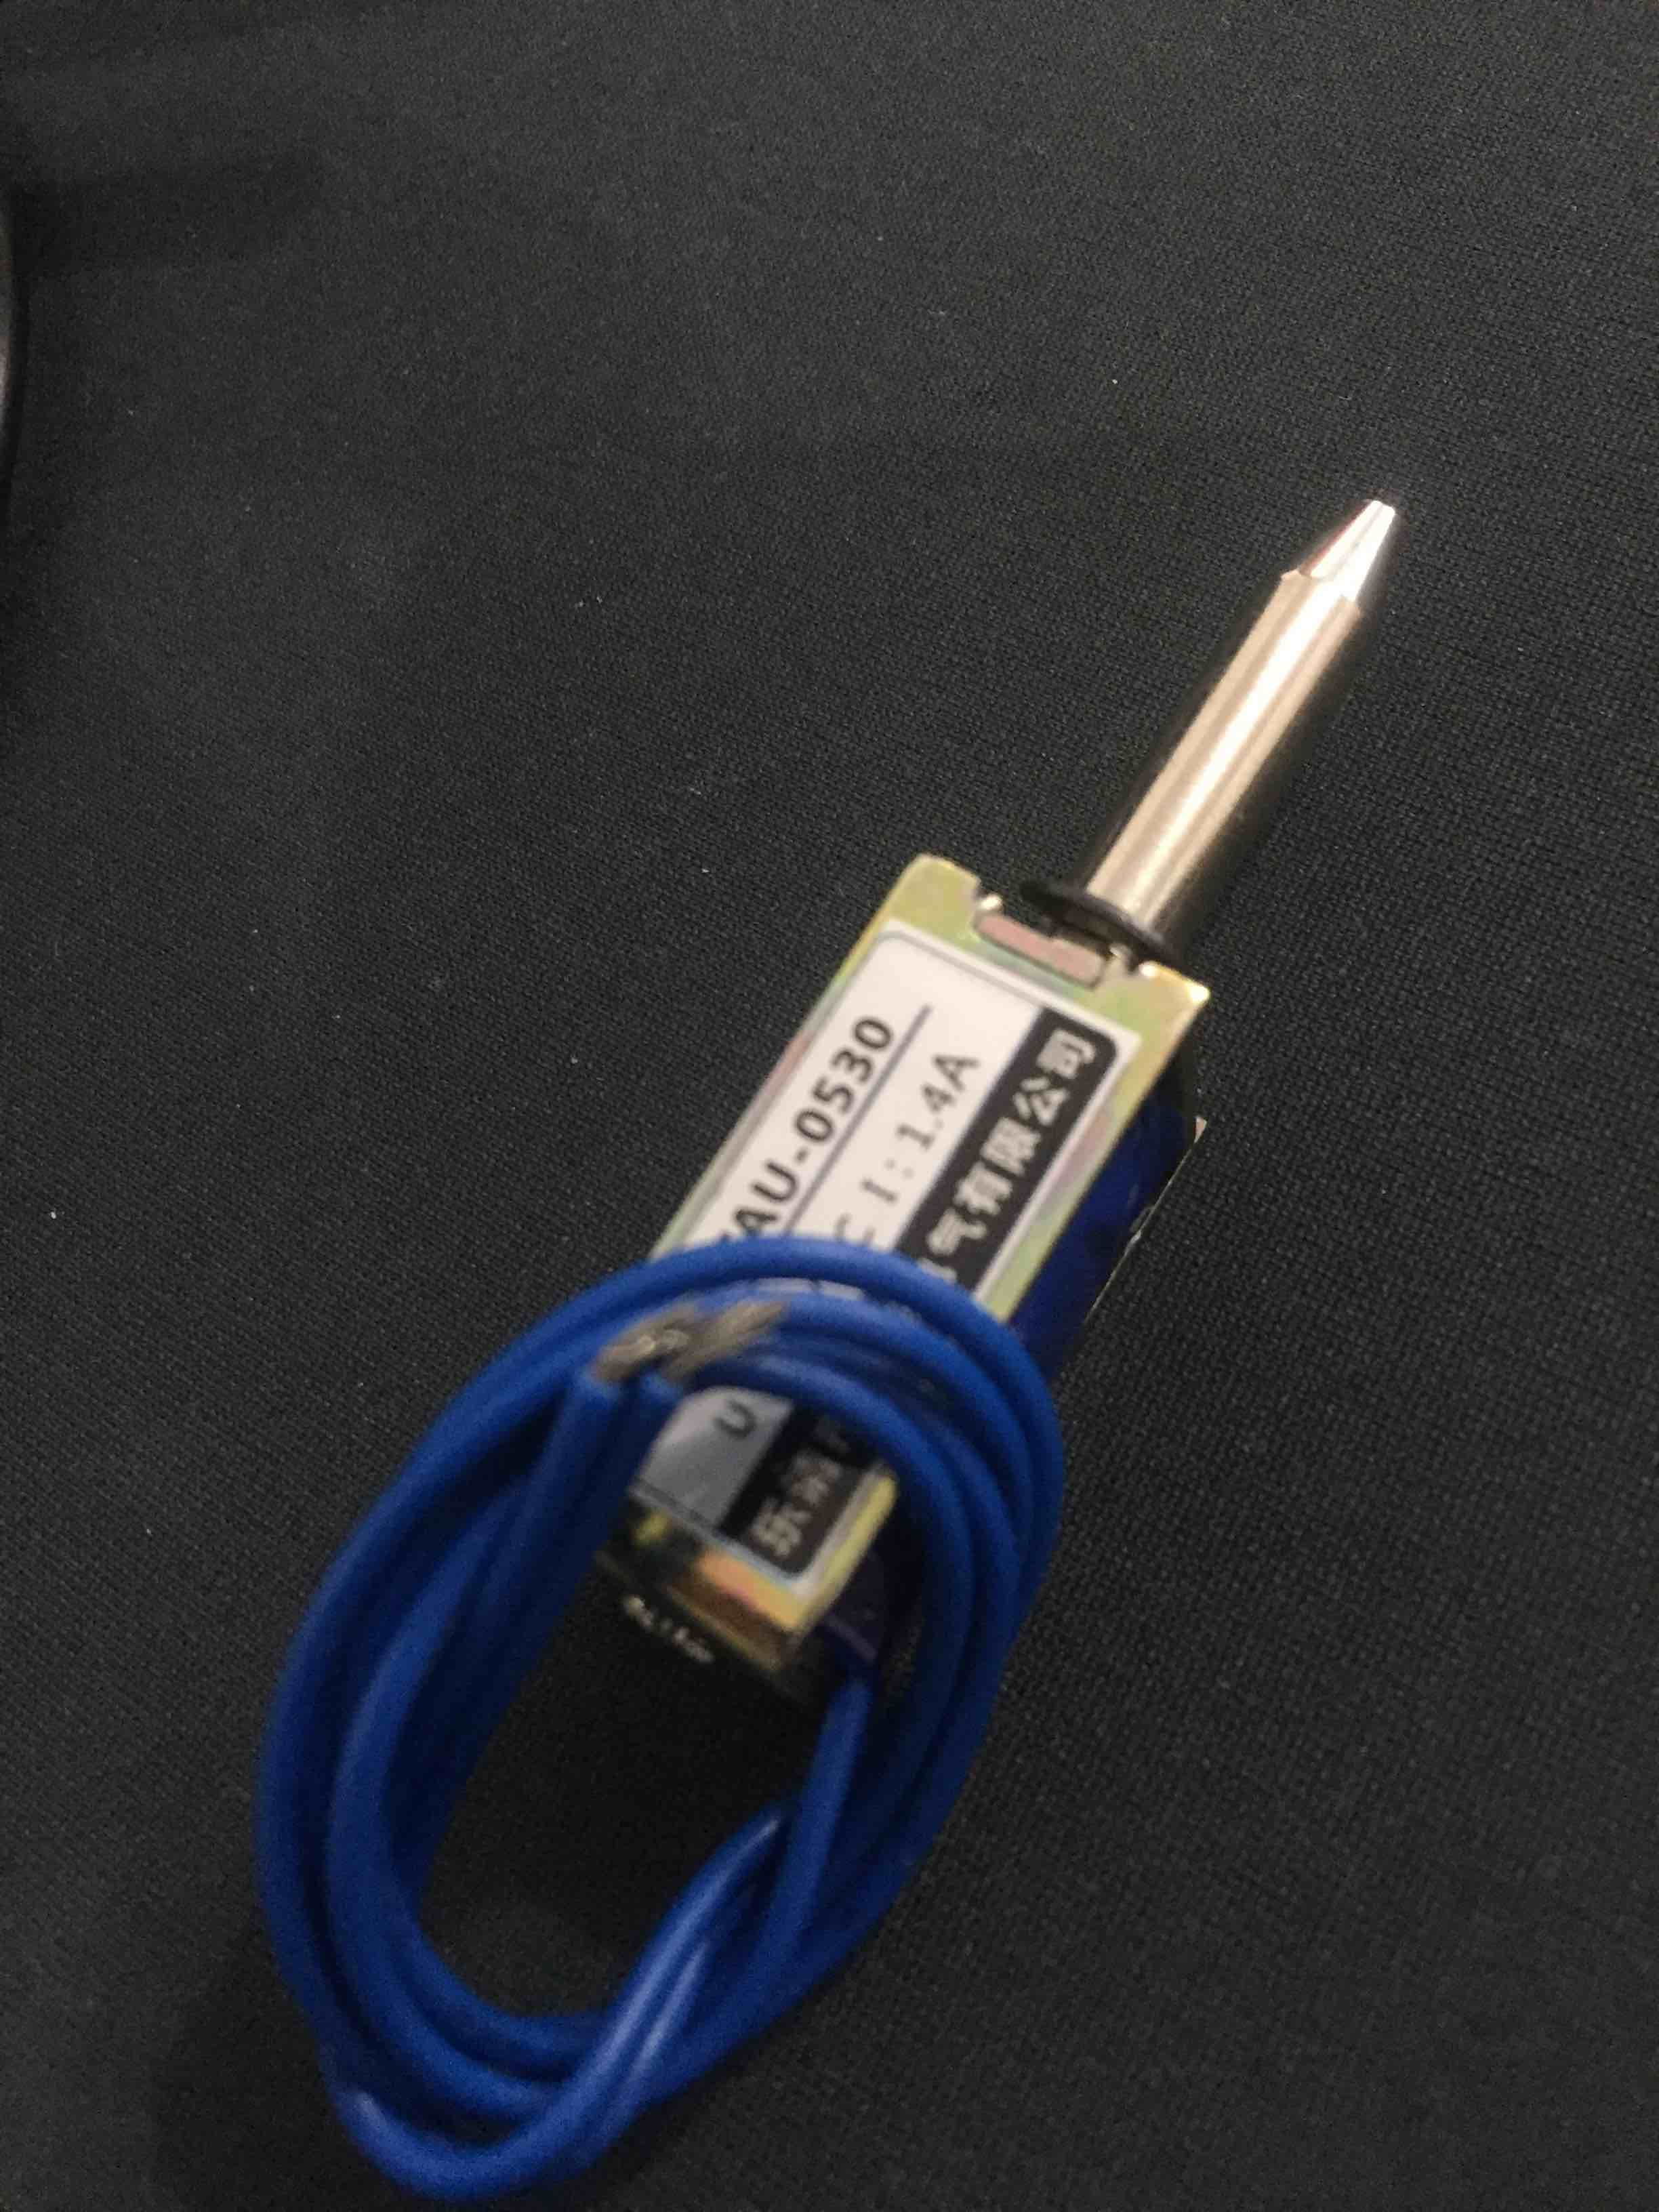
\includegraphics[scale= 0.06]{figuras/solenoide.jpg}
            \caption{Solenoide utilizado.}
            \label{solenoide}
\end{figure}

	
\section{Relatório de teste}



